\chapter{Sprint 3 "Demande de payout, statistiques et signalement d'erreurs"}

\section*{Introduction}
Dans ce chapitre, nous examinerons le dernier sprint, qui suit les mêmes étapes que le précédent. Nous débuterons par un extrait du backlog du sprint 3, puis passerons aux spécifications fonctionnelles, à la conception, à la revue du sprint, et conclurons par une rétrospective.

\section{ Extrait du backlog du sprint 3}
Les thèmes du sprint sont : La gestion des demandes de payout, dashboard statistique, le système de notifications, ainsi que la gestion des signalements d'erreurs et des feedbacks. \\
Nous allons maintenant présenter un extrait du sprint backlog à travers le user story : "En tant que développeur, je veux pouvoir consulter les statistiques de consommation de mes APIs "

\begin{table}[H]
    \centering
    \caption{Extrait du backlog du sprint3 "Statistiques de consommation de mes API"}
    \label{tab:task_estimation_statistics}
    \begin{longtable}{|p{0.25\linewidth}|p{0.25\linewidth}|p{0.35\linewidth}|p{0.15\linewidth}|}
        \hline
        \textbf{User story} & \textbf{Tâches} & \textbf{Sous-tâches} & \textbf{Estimation} \\
        \hline
        \endfirsthead
        \multicolumn{4}{c}%
        {{\bfseries \tablename\ \thetable{} -- suite de la page précédente}} \\
        \hline
        \textbf{User story} & \textbf{Tâches} & \textbf{Sous-tâches} & \textbf{Estimation} \\
        \hline
        \endhead
        \hline \multicolumn{4}{|r|}{{\bfseries Suite à la page suivante}} \\
        \hline
        \endfoot
        \hline
        \endlastfoot

        \multirow{8}{=}{En tant que développeur, je veux pouvoir consulter les statistiques de consommation de mes APIs.}
            & Préparation de la maquette & Réalisation de la maquette & 2h \\
        \cline{2-4}
            & \multirow{1}{=}{Modélisation \& conception UML} & Réalisation du diagramme de séquence & 2h \\
        \cline{2-4}
            & \multirow{2}{=}{Préparation du backend} & Réalisation de la fonction get "getConsumerAnalytics" & 3h \\
        \cline{3-4}
            & & Test & 2h \\
        \cline{2-4}
            & \multirow{4}{=}{Préparation du frontend} & Réalisation de l'interface & 2h \\
        \cline{3-4}
            & & Préparation du service "StatisticService" & 1h 30min \\
        \cline{3-4}
            & & Préparation de la fonction “createConsumerLineChart” & 1h 30min \\
        \cline{3-4}
            & & Test & 30min \\
        \hline
    \end{longtable}
\end{table}

\pagebreak

\section{ Spécification fonctionnelle}
Dans cette partie, nous allons présenter le diagramme de cas d'utilisation du sprint 3 et un exemple de maquette.

\subsection{Diagramme de cas d'utilisation}
Dans cette partie, nous allons présenter le diagramme de cas d'utilisation du sprint 3. \\
Les cas d'utilisation suivants ont été intégrés au sprint 3.

\begin{itemize}
    \item  \textbf{Développeur}
    \begin{itemize}
        \item  Consulter mes statistiques.
        \item Consulter mes transactions.
        \item Gérer mes feedbacks.
        \item Consulter mes notifications.
        \item Gérer les signalements.
    \end{itemize}
    \item  \textbf{Administrateur}
    \begin{itemize}
        \item Gérer les demandes de payout.
        \item Consulter les statistiques.
        \item Consulter les signalements.
        \item Consulter mes notifications.
    \end{itemize} 
   
\end{itemize}
Un acteur secondaire a été introduit au niveau de ce sprint :
\begin{itemize}
\item \textbf{Paypal} pour la réalisation du payout.
\end{itemize} 
\pagebreak


\begin{figure}[H]
    \centering
    \frame{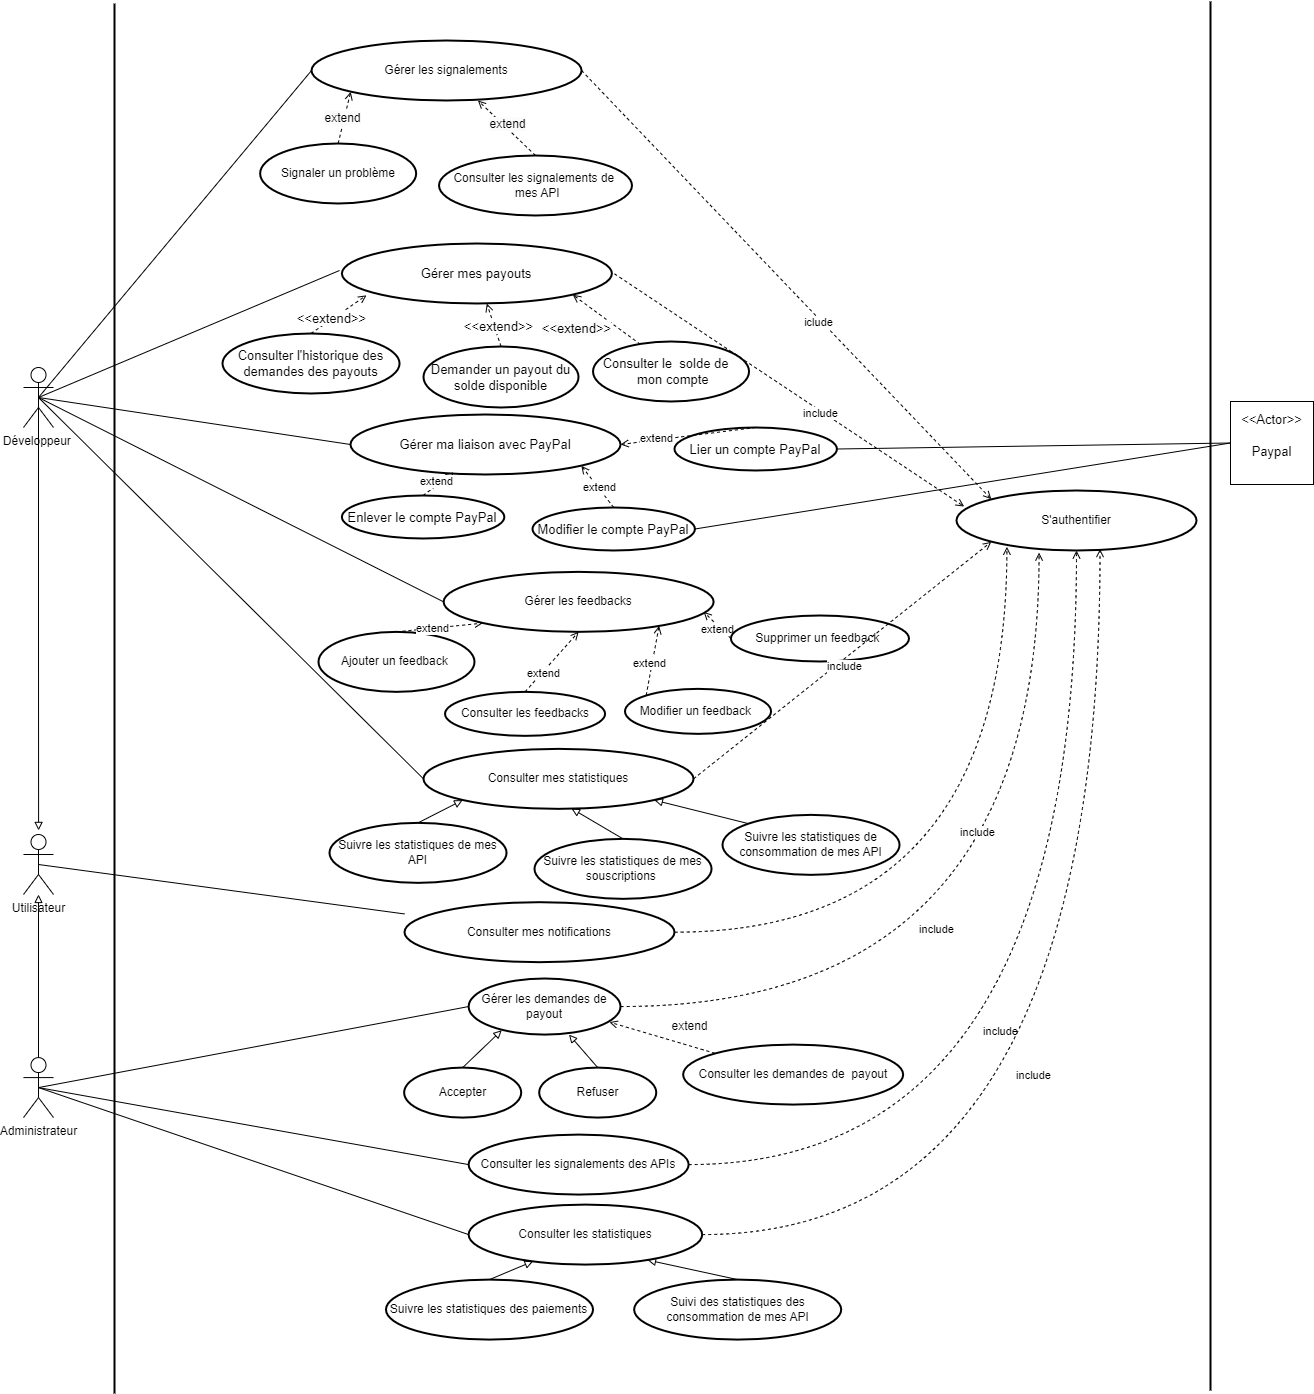
\includegraphics[width=1.1\columnwidth]{diagrammedecasdutilisationensprint3.png}}
    \caption{Diagramme de cas d'utilisation du sprint 3 }
    \label{fig:logo_tt}
\end{figure}

\pagebreak
\subsection{Exemple d'une maquette d'interface du sprint 3}

La figure suivante représente la maquette du tableau de bord de statistique des payouts réalisés dans la marketplace.
\begin{figure}[H]
    \centering
    \frame{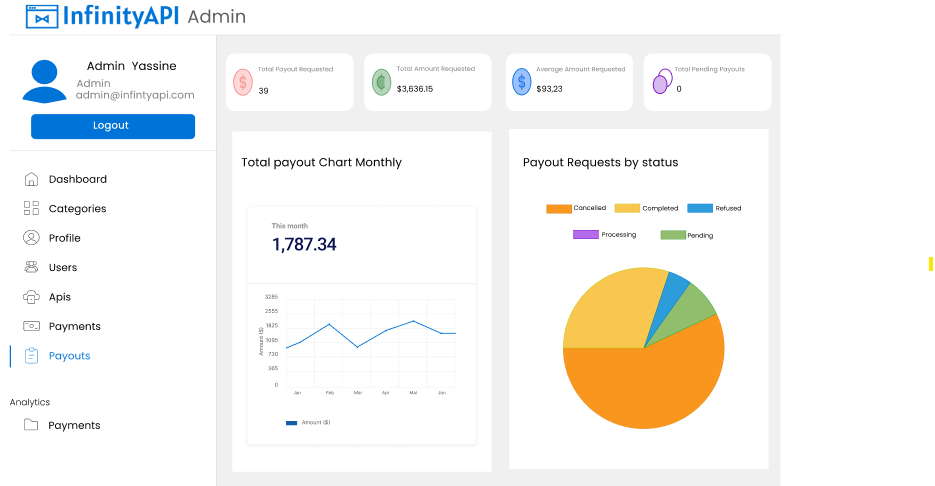
\includegraphics[width=1.1\columnwidth]{interfacedestatistiquedespayout.png   }}
    \caption{Maquette de statistiques des payouts réalisés sur la plateforme   }
    \label{fig:logo_tt}
\end{figure}
\pagebreak

\section{ Conception}
Dans cette partie, nous allons présenter la modélisation structurelle à travers le diagramme de classes et le diagramme de déploiement avant de présenter les principaux traitements de sprint relatifs à :
\begin{itemize}	
   \item La demande de payout
   \item L'ajout d'un rapport 
   \item L'ajout  de statistiques détaillé en annexe 1 
\end{itemize}
\subsection{Modélisation structurelle}
\subsubsection{Diagramme du classes}

\textbf{a. Règles de gestion et calcul} \\
Voici les principales règles de gestion avant de présenter le diagramme de classes :

    \begin{itemize}
        \item  Un développeur peut soumettre zéro ou plusieurs feedbacks.
        \item Chaque feedback est soumis par un seul développeur.
        \item Un feedback est relatif à une API.
        \item Une API peut avoir zéro ou plusieurs feedbacks.
        \item Un développeur peut avoir zéro ou plusieurs notifications.
        \item Chaque notification est associée à  un seul développeur.
        \item Un développeur peut signaler zéro ou plusieurs rapports.
        \item Chaque rapport est signalé par un seul développeur.
        \item Un développeur peut réaliser zéro ou plusieurs payouts.
        \item Chaque payout est réalisé par un seul développeur.

    \end{itemize}
\pagebreak

\textbf{b. Diagramme de classes } \\

\begin{figure}[H]
    \centering
    \frame{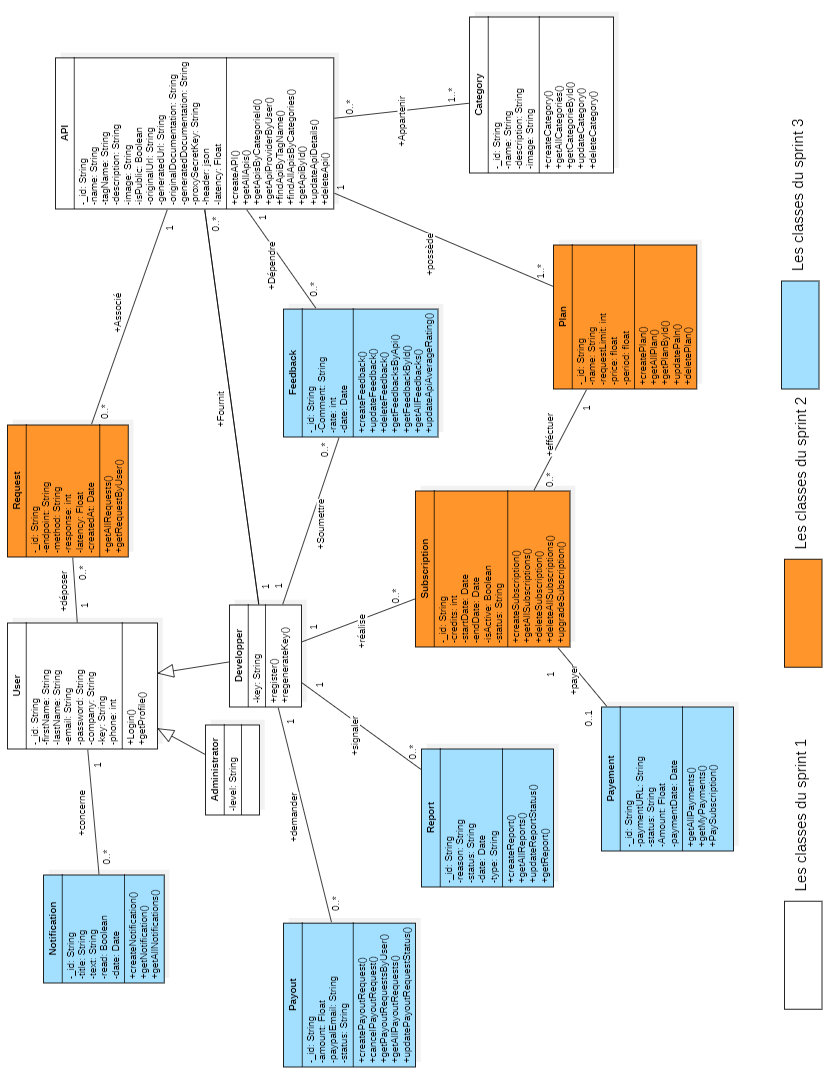
\includegraphics[width=1\columnwidth]{Diagrammedeclassedesprint3.png    }}
    \caption{Diagramme de classes du sprint 3    }
    \label{fig:logo_tt}
\end{figure}
La représentation NoSql associée à notre base de données est présentée en annexe 1

\subsubsection{Diagramme de déploiement}

Le diagramme de déploiement illustre l'architecture de l'application "InfinityAPI", montrant les interactions entre ses différents composants. Le client utilise un navigateur web pour accéder à l'application via HTTP/HTTPS. Le serveur web héberge l'interface utilisateur (InfinityAPI Frontend) et communique avec le servec backend de l'application (InfinityAPI Backend) fonctionnant dans un environnement Node.js. Le backend communique avec les fournisseurs de services API externes et les passerelles de paiement, Stripe et PayPal, également via HTTP/HTTPS, pour gérer les transactions financières. Pour le stockage et la récupération des données, le backend utilise une base de données MongoDB hébergée sur MongoDB Atlas, accessible via TCP/IP. Cette architecture assure une interaction fluide entre le client, les services externes, et la base de données, tout en maintenant la sécurité et l'efficacité des transactions et des traitements de données.
\begin{figure}[H]
    \centering
    \frame{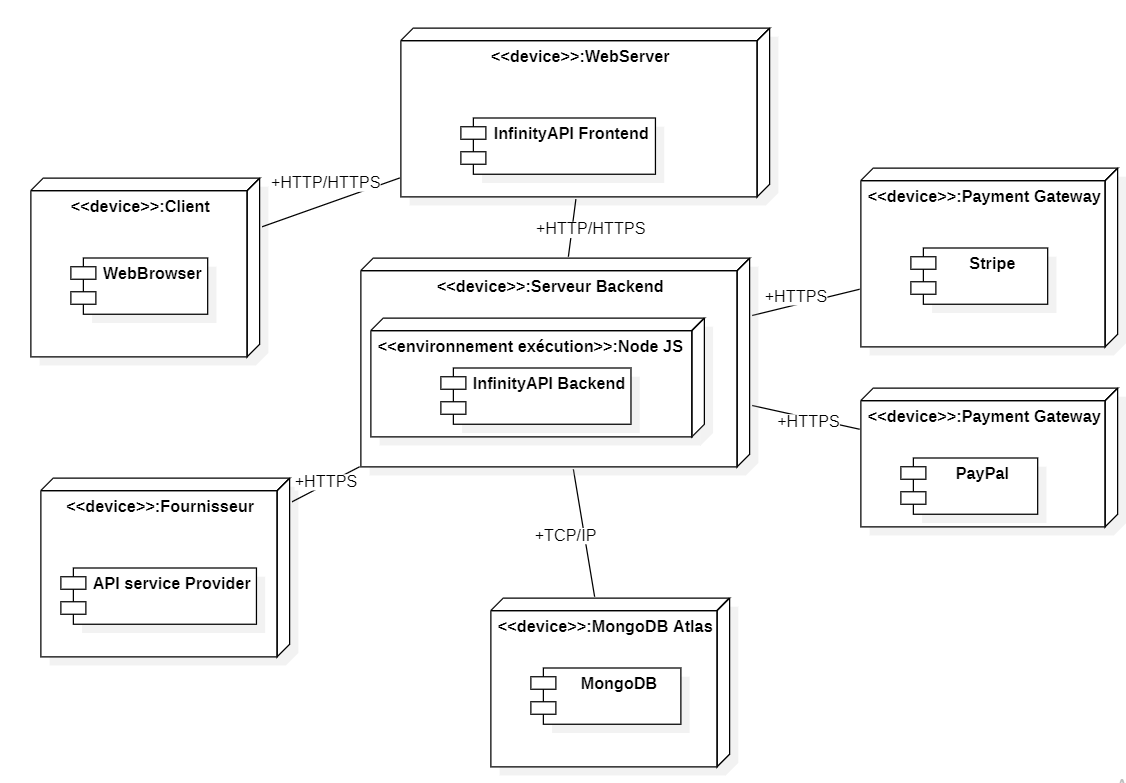
\includegraphics[width=1\columnwidth]{diagrammededeploiement.png}}
    \caption{Diagramme de déploiement}
    \label{fig:logo_tt}
\end{figure}
\pagebreak

\subsection{Diagramme d'état "Demande d'un payout"}
Le processus de demande de payout passe par plusieurs états :
\begin{itemize}
    \item \textbf{Pending (En attente) :} Cet état est atteint lorsque le développeur crée une demande de payout. La demande est en attente d'acceptation ou de rejet par l'administrateur.
    \item \textbf{Processing (En cours de traitement) :} Cet état indique que la demande de payout a été acceptée et est actuellement en cours de traitement par l'administrateur.
    \item \textbf{Completed (Terminée) :} Cet état indique que la demande de payout a été complétée avec succès. L'administrateur a finalisé le traitement de la demande.
    \item \textbf{Refused (Refusée) :} Cet état indique que la demande de payout a été rejetée par l'administrateur.
    \item \textbf{Cancelled (Annulée) :} Cet état indique que la demande de payout a été annulée par le développeur avant ou durant le traitement.
\end{itemize}
La figure suivante illustre le diagramme d’état relatif à une demande de payout.
\begin{figure}[H]
    \centering
    \frame{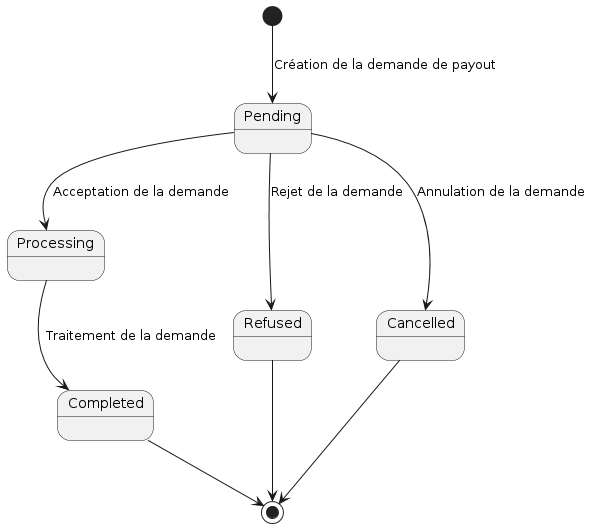
\includegraphics[width=0.9\columnwidth]{digrammedetatsouscription.png}}
    \caption{Diagramme d'état "Demande d'un payout"}
    \label{fig:logo_tt}
\end{figure}

\pagebreak

\subsection{Diagramme de séquence "Demande de payout"}
Ce diagramme de séquence illustre les interactions entre les différents composants de la marketplace lors d'une demande de solde(payout request). Tout d'abord, le développeur soumet un payout request. Une requête HTTP est alors envoyée au backend, qui vérifie la validité du jeton d'authentification. Si le jeton est invalide, un message d'erreur "invalid token" est renvoyé. Si le jeton est valide, le backend vérifie si le compte du développeur est lié à un compte PayPal. Si ce n'est pas le cas, un message d'erreur "You have no linked PayPal account" est affiché. Si le compte PayPal est lié, le backend vérifie si le solde du compte est supérieur à 0et si la dernière demande de paiement date de plus de 30 jours. Si toutes ces conditions sont remplies, la demande de paiement est acceptée, le solde du compte est mis à jour à zéro, et un message de succès est affiché pour indiquer que la demande de paiement a été ajoutée avec succès.

\begin{figure}[H]
    \centering
    \frame{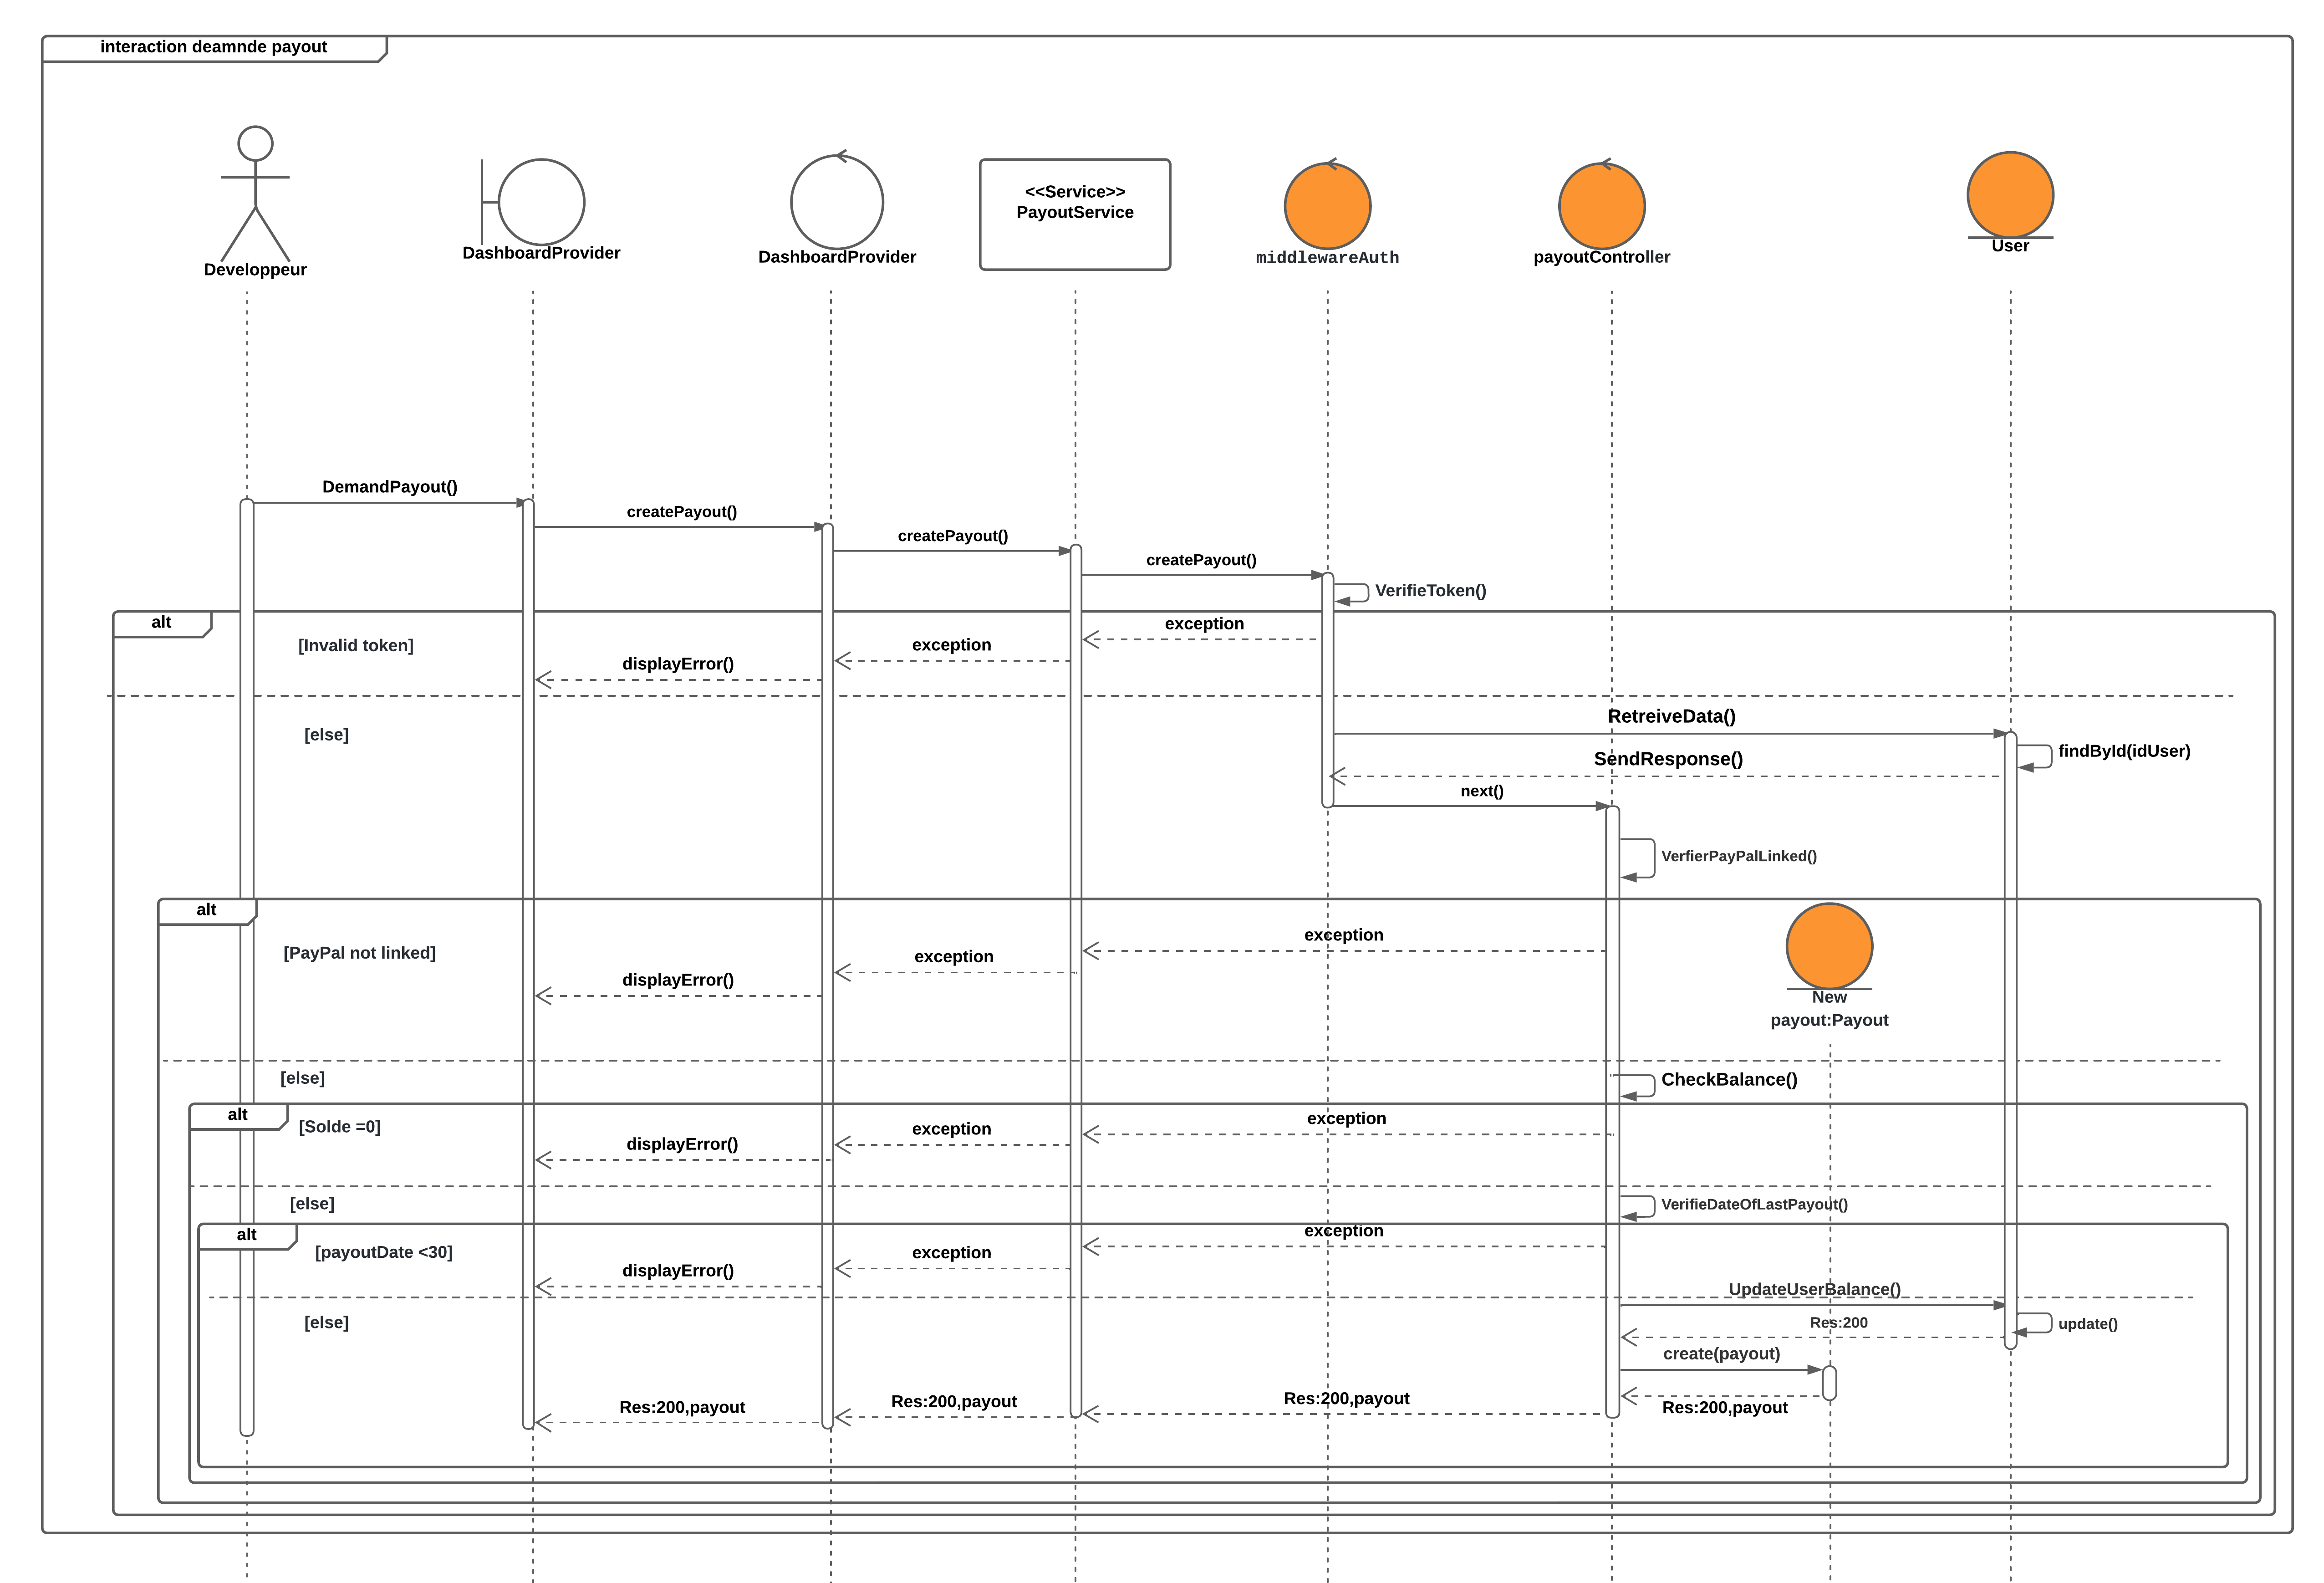
\includegraphics[width=1.1\columnwidth]{diagrammedesequencepayoutrequest.png }}
    \caption{Diagramme de séquence "Demande de payout" }
    \label{fig:logo_tt}
\end{figure}
\pagebreak



\subsection{Diagramme de séquence "Ajouter rapport"}
Ce diagramme de séquence illustre l'enchaînement des interactions entre les différents composants de la marketplace pour l'ajout d'un rapport signalant une erreur. Le développeur remplit le formulaire d'ajout d’un signalement. Si les champs sont invalides, un message d'erreur est affiché. Sinon, une requête HTTP est envoyée au backend. Le backend vérifie alors la validité du jeton. Si le jeton est invalide, un message d'erreur "invalid token" est renvoyé. Sinon, un message de succès est affiché pour indiquer que le rapport a été ajouté avec succès.

\begin{figure}[H]
    \centering
    \frame{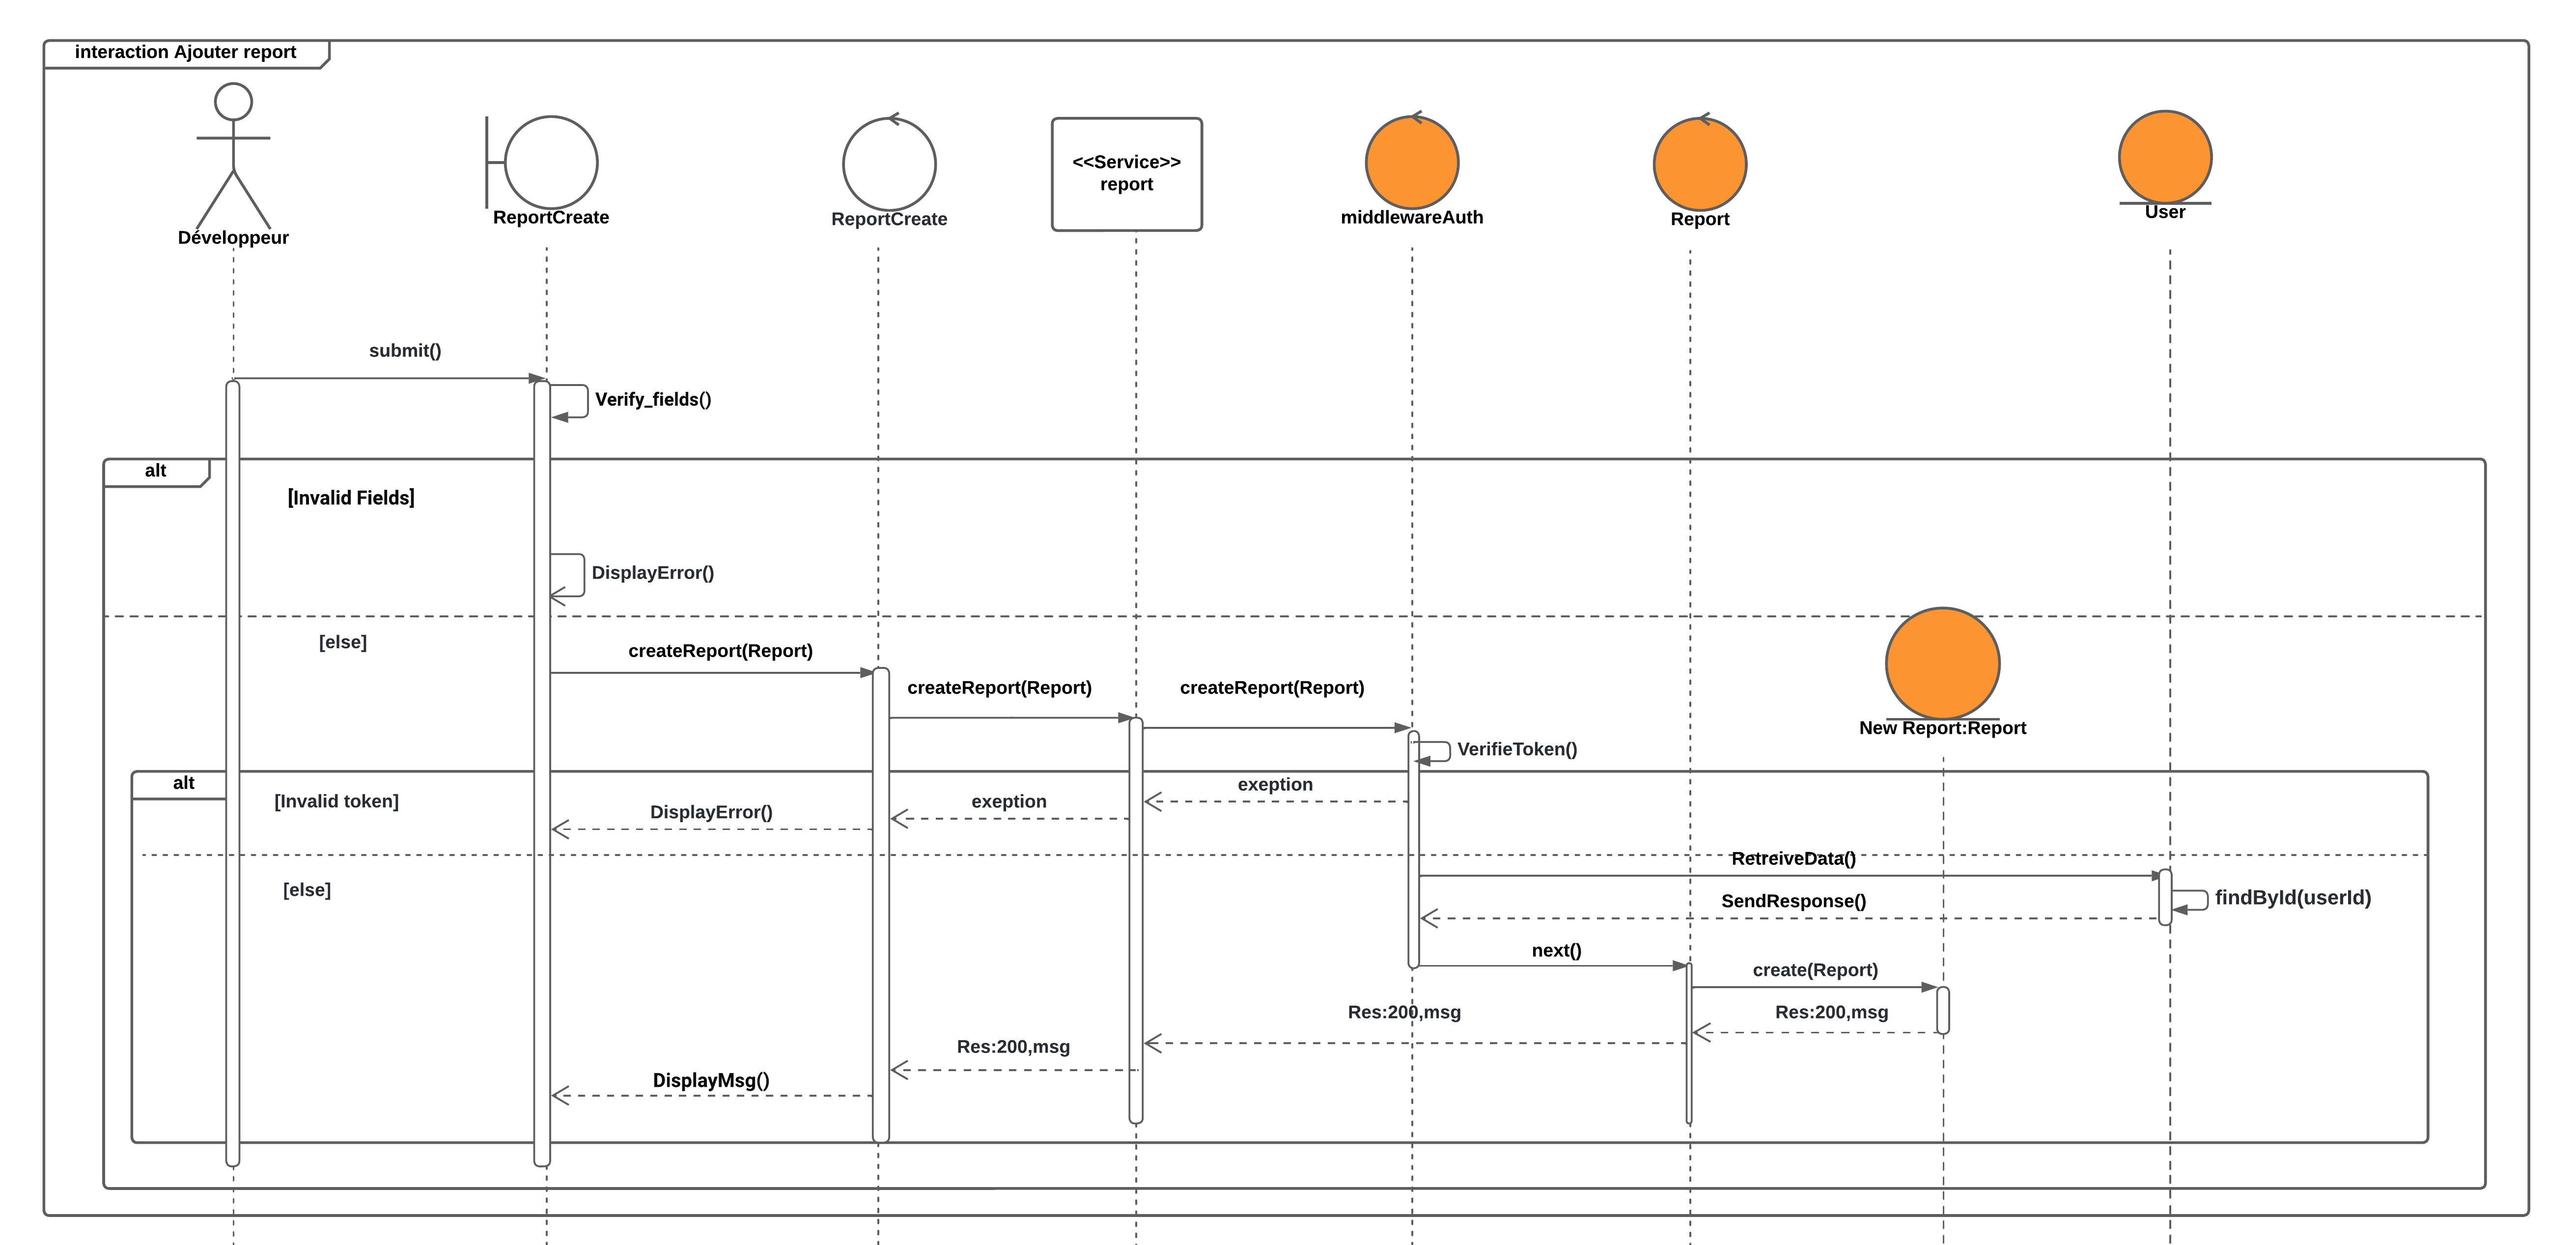
\includegraphics[width=1.1\columnwidth]{diagrammedesequenceAjouterReport.png  }}
    \caption{Diagramme de séquence "Ajouter rapport"    }
    \label{fig:logo_tt}
\end{figure}






\section{ Revue de sprint }
Dans cette partie, nous allons exposer le travail réalisé durant le sprint 3, ainsi que le
burndown chart et la rétrospective.
    \subsection{Réalisation}
    Dans cette étape, nous allons explorer les principales interfaces réalisées lors de ce sprint.
    \pagebreak
    \subsubsection{Gestion des demandes de payout}
    Cette interface représente le processus de demande d'un payout.
    \begin{figure}[H]
        \centering
        \frame{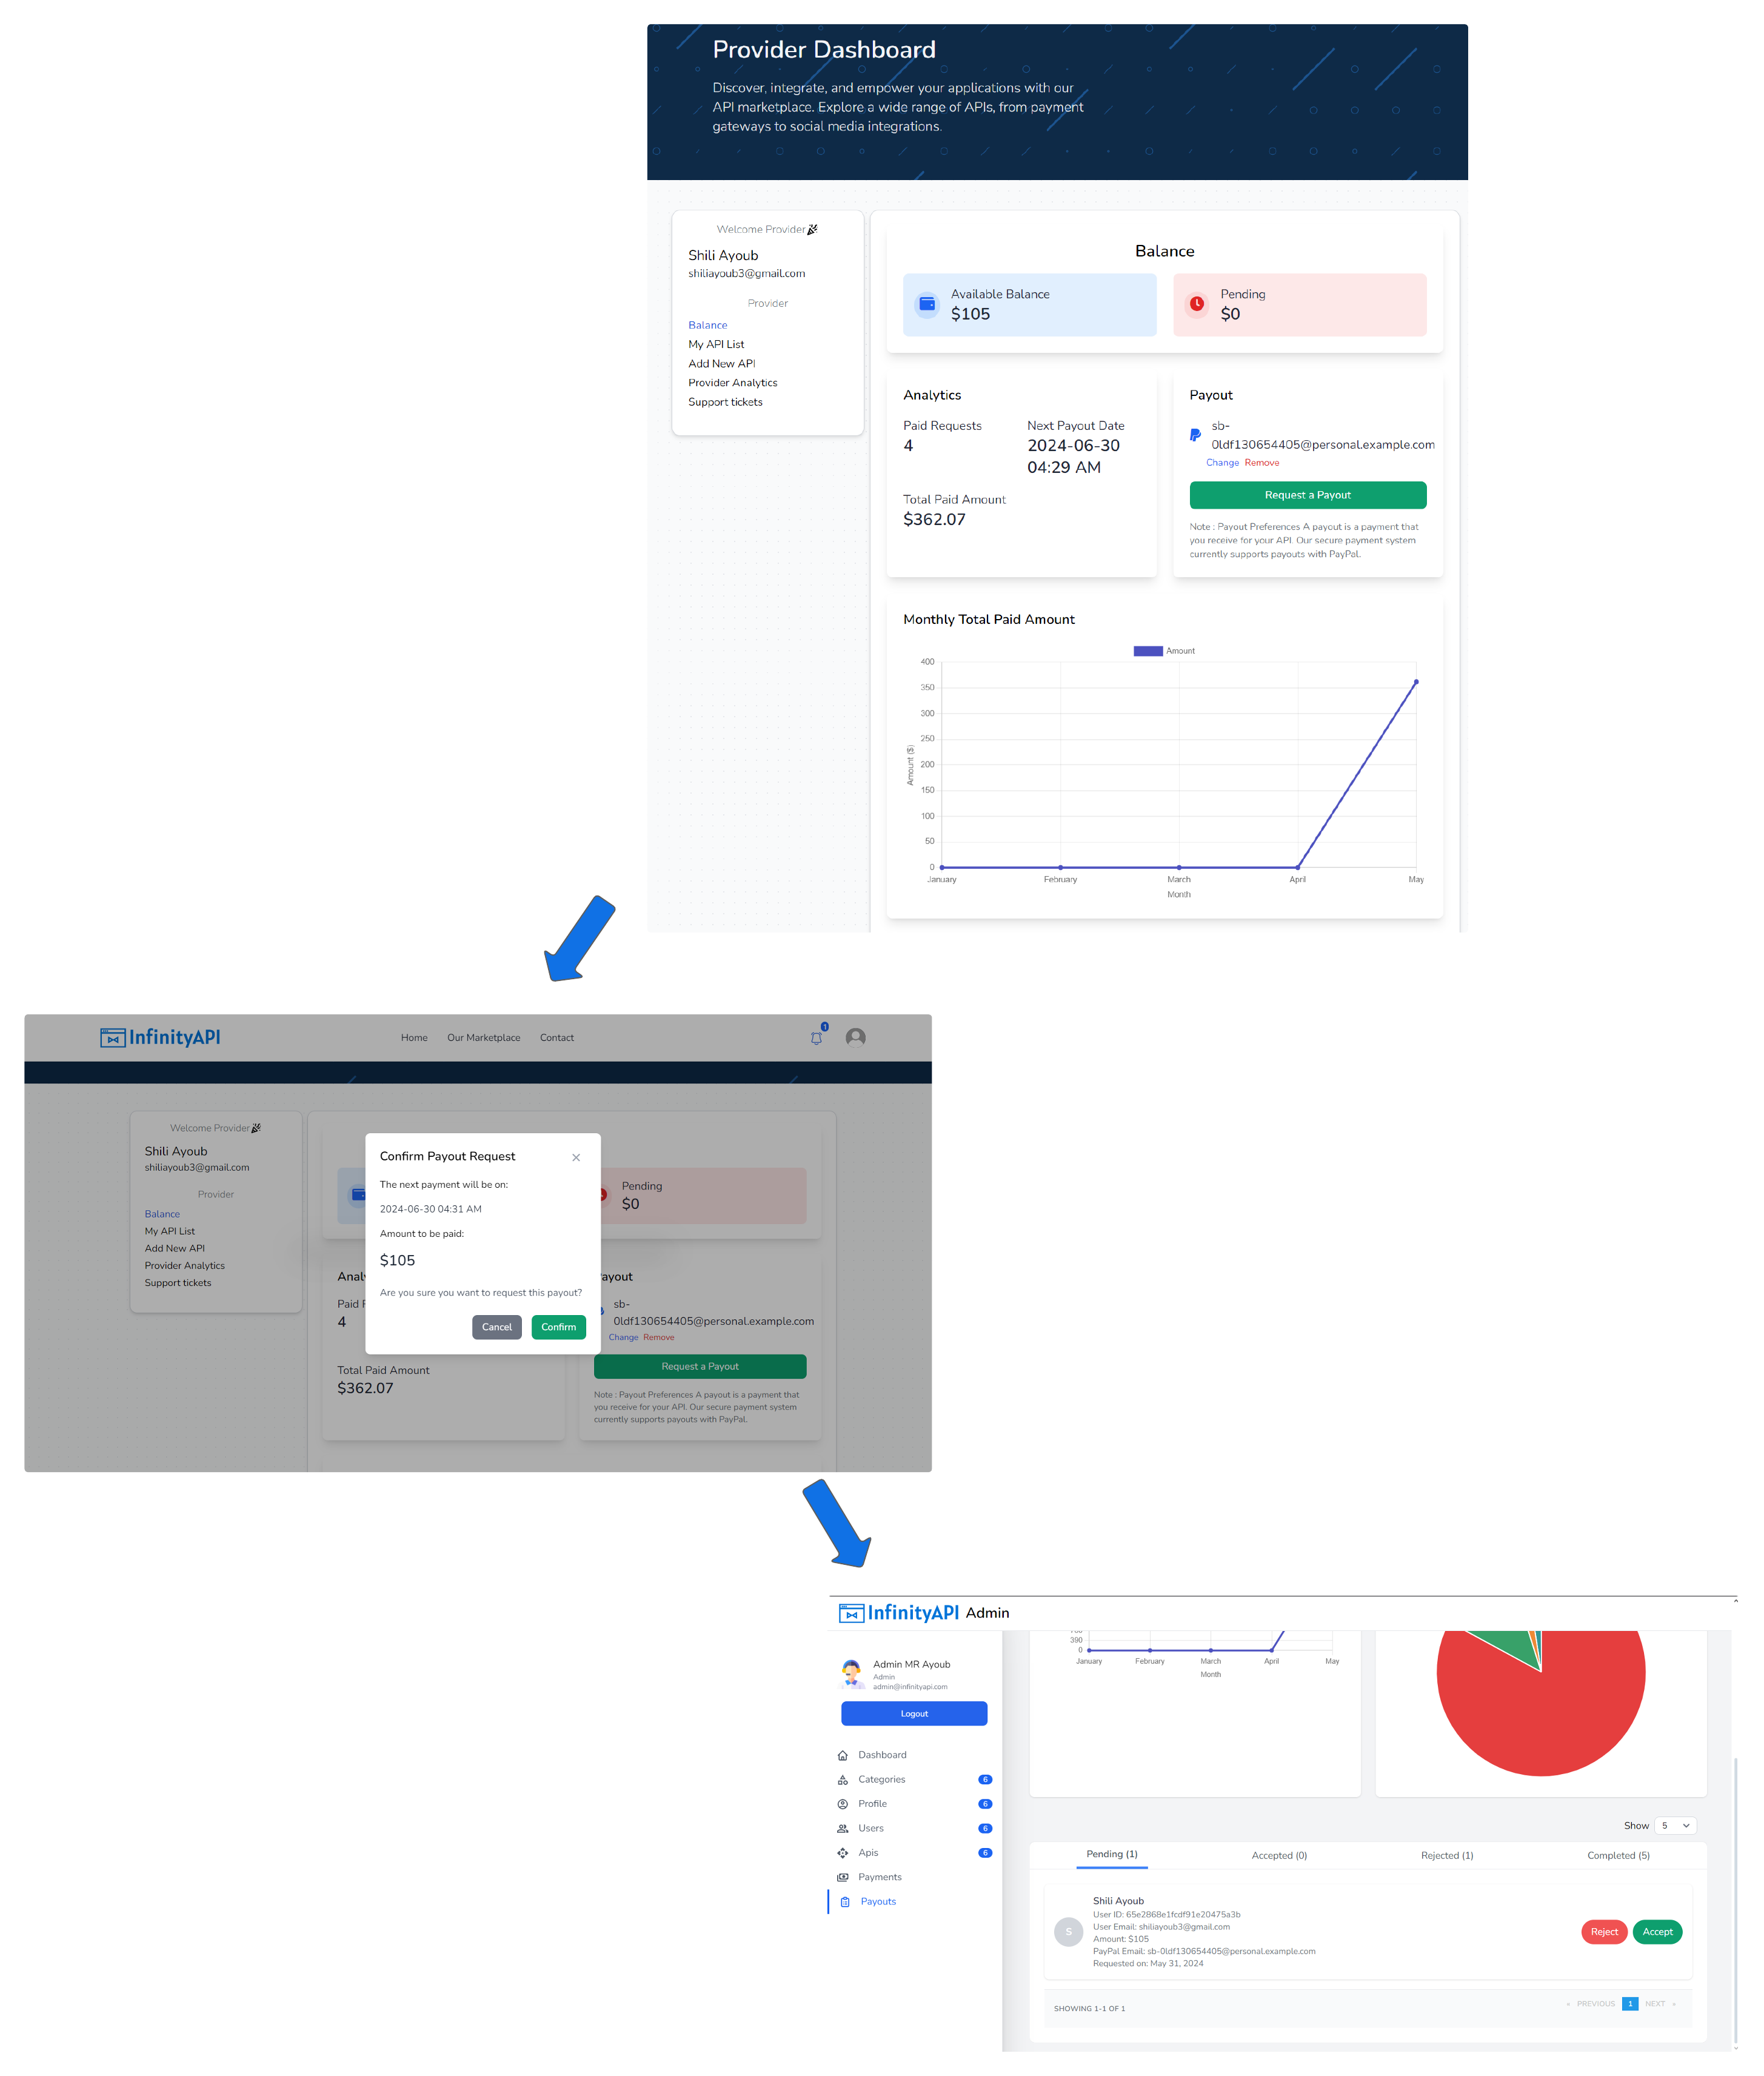
\includegraphics[width=1.1\columnwidth]{processusdepayout.png}}
        \caption{Interface du processus de payout  }
        \label{fig:logo_tt}
    \end{figure}

    \subsubsection{Dashboard de statistiques}
    Cette interface ,destinée au fournisseur d'API, affiche les statistiques des souscriptions, des requêtes et de la latence de ses API. 
    \begin{figure}[H]
        \centering
        \frame{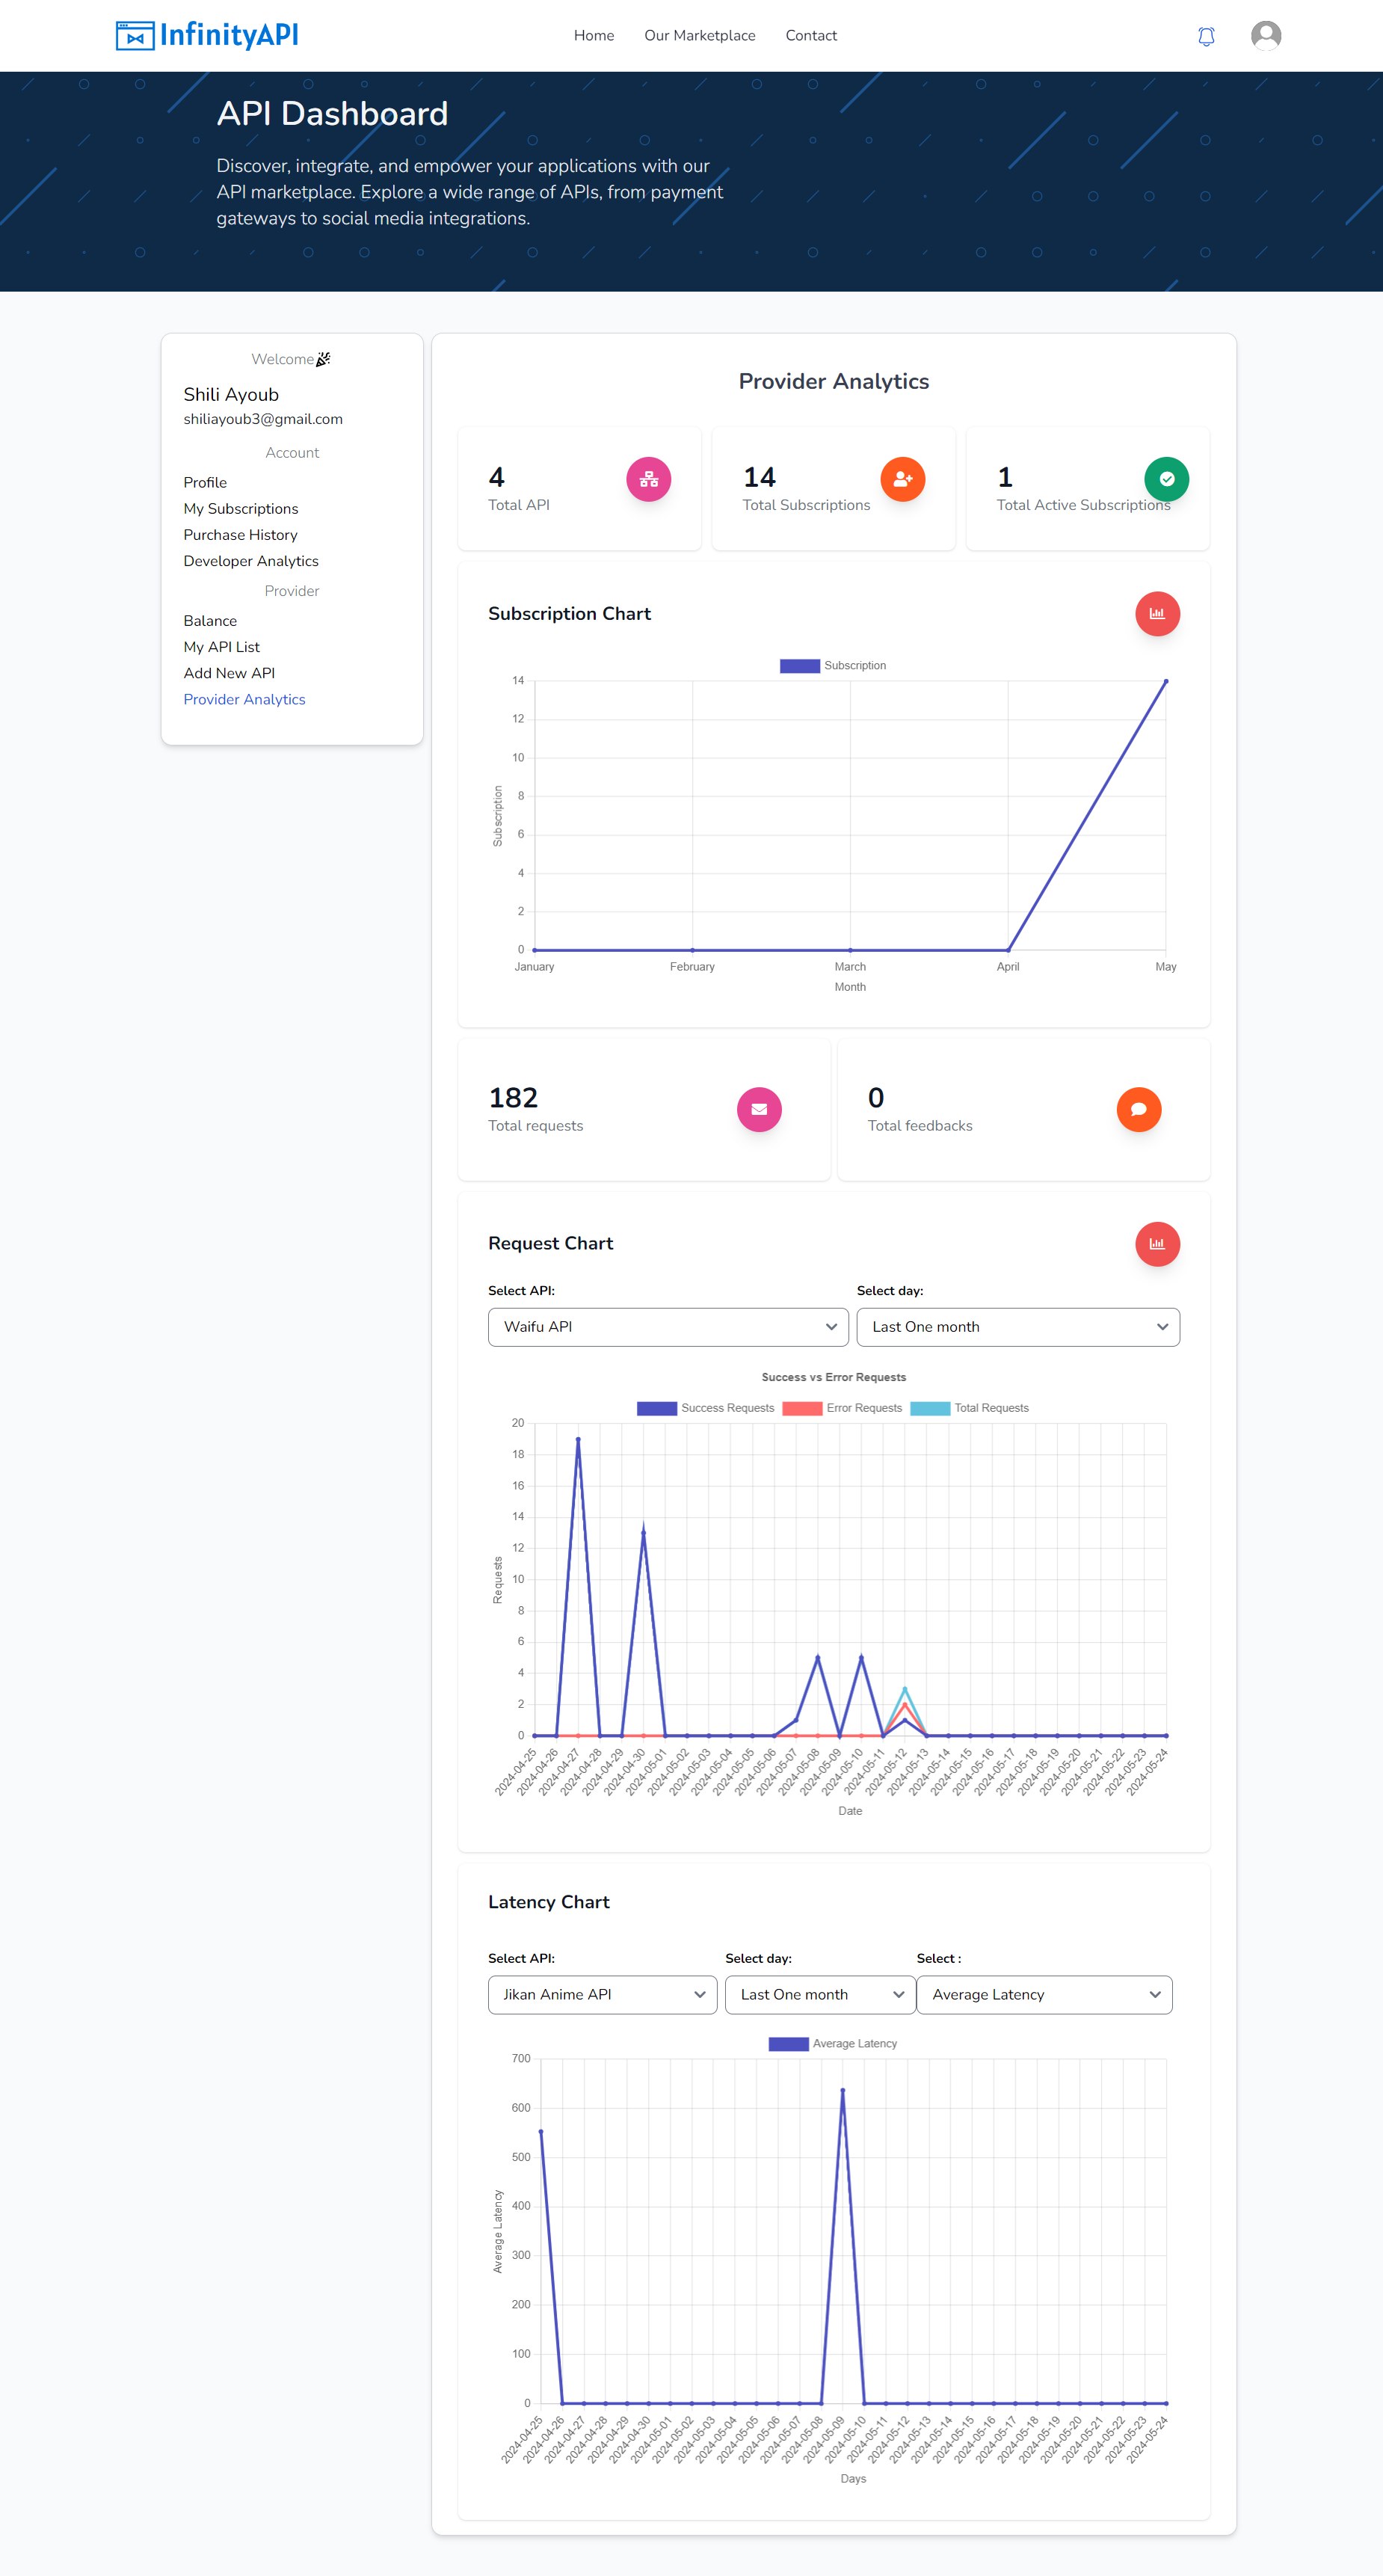
\includegraphics[width=0.7\columnwidth]{ InterfaceduproviderdeAPI.png}}
        \caption{ Interface du fournisseur d'API }
        \label{fig:logo_tt}
    \end{figure}


    Cette interface affiche deux statistiques de paiement effectuées dans la marketplace par mois et par catégorie.
    \begin{figure}[H]
        \centering
        \frame{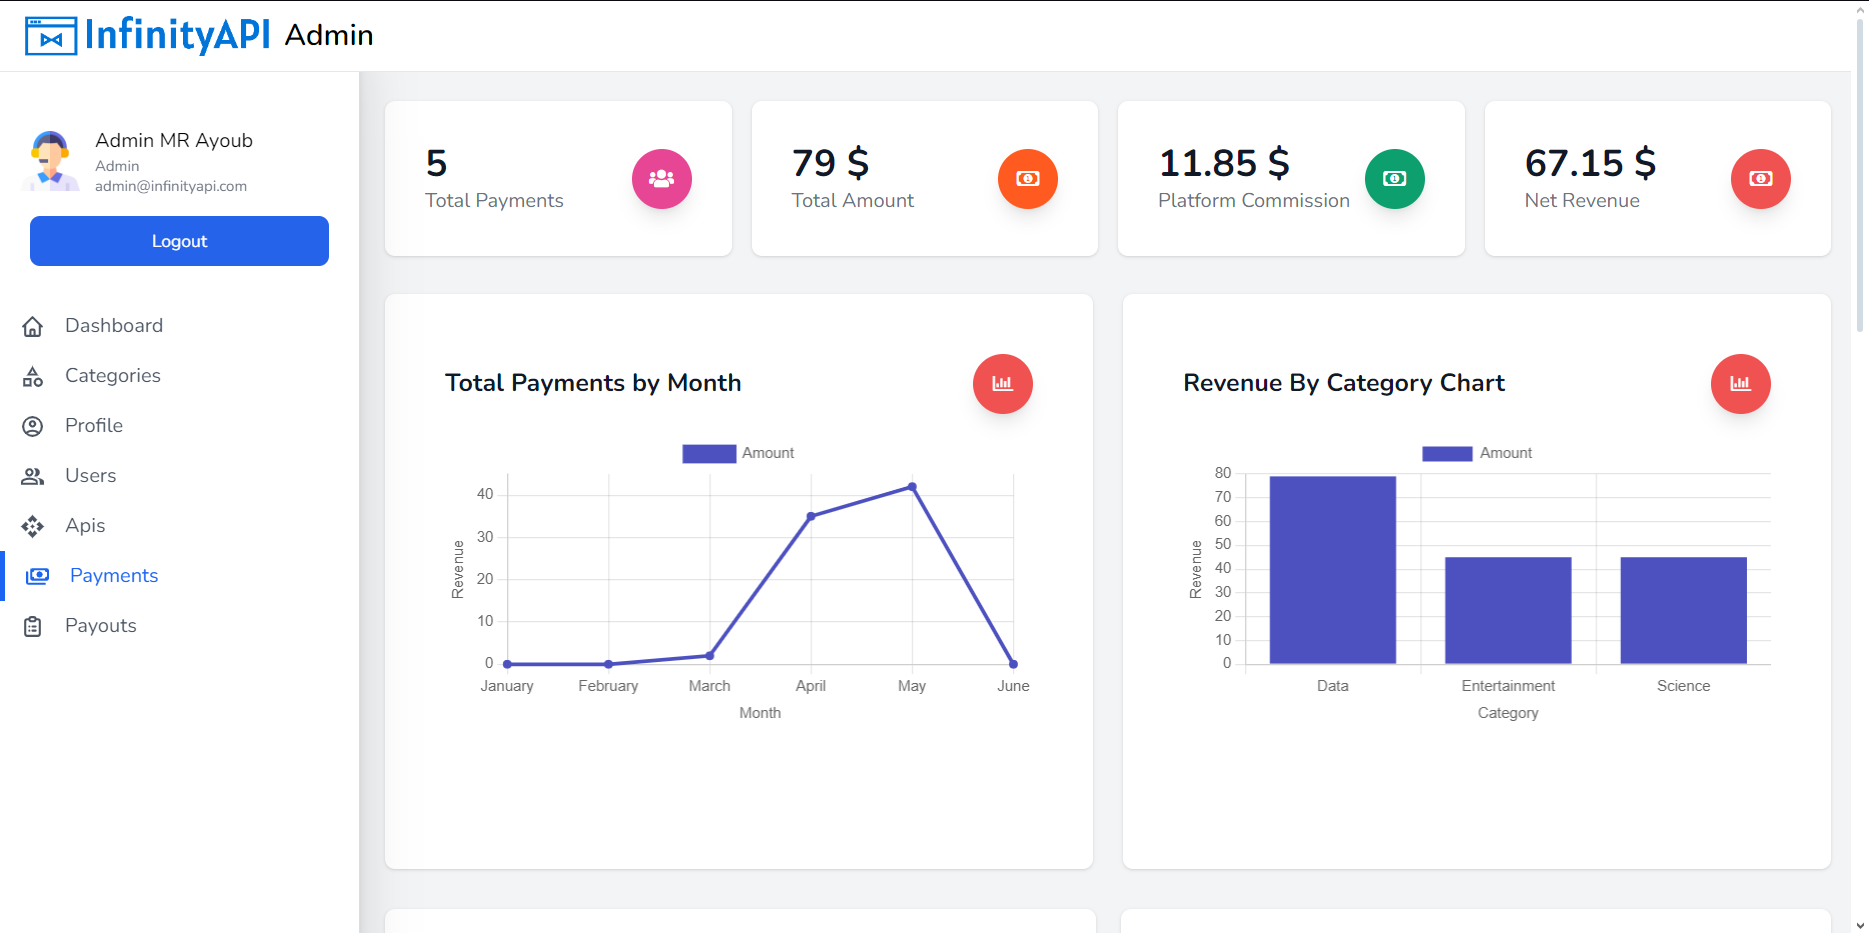
\includegraphics[width=1\columnwidth]{interfacedestatistiquedespayement.png }}
        \caption{ Interface du statistique de paiement }
        \label{fig:logo_tt}
    \end{figure}

    \subsubsection{Gestion des feedbacks}

    Cette interface représente le processus de l'ajout d'un feedback 
    \begin{figure}[H]
        \centering
        \frame{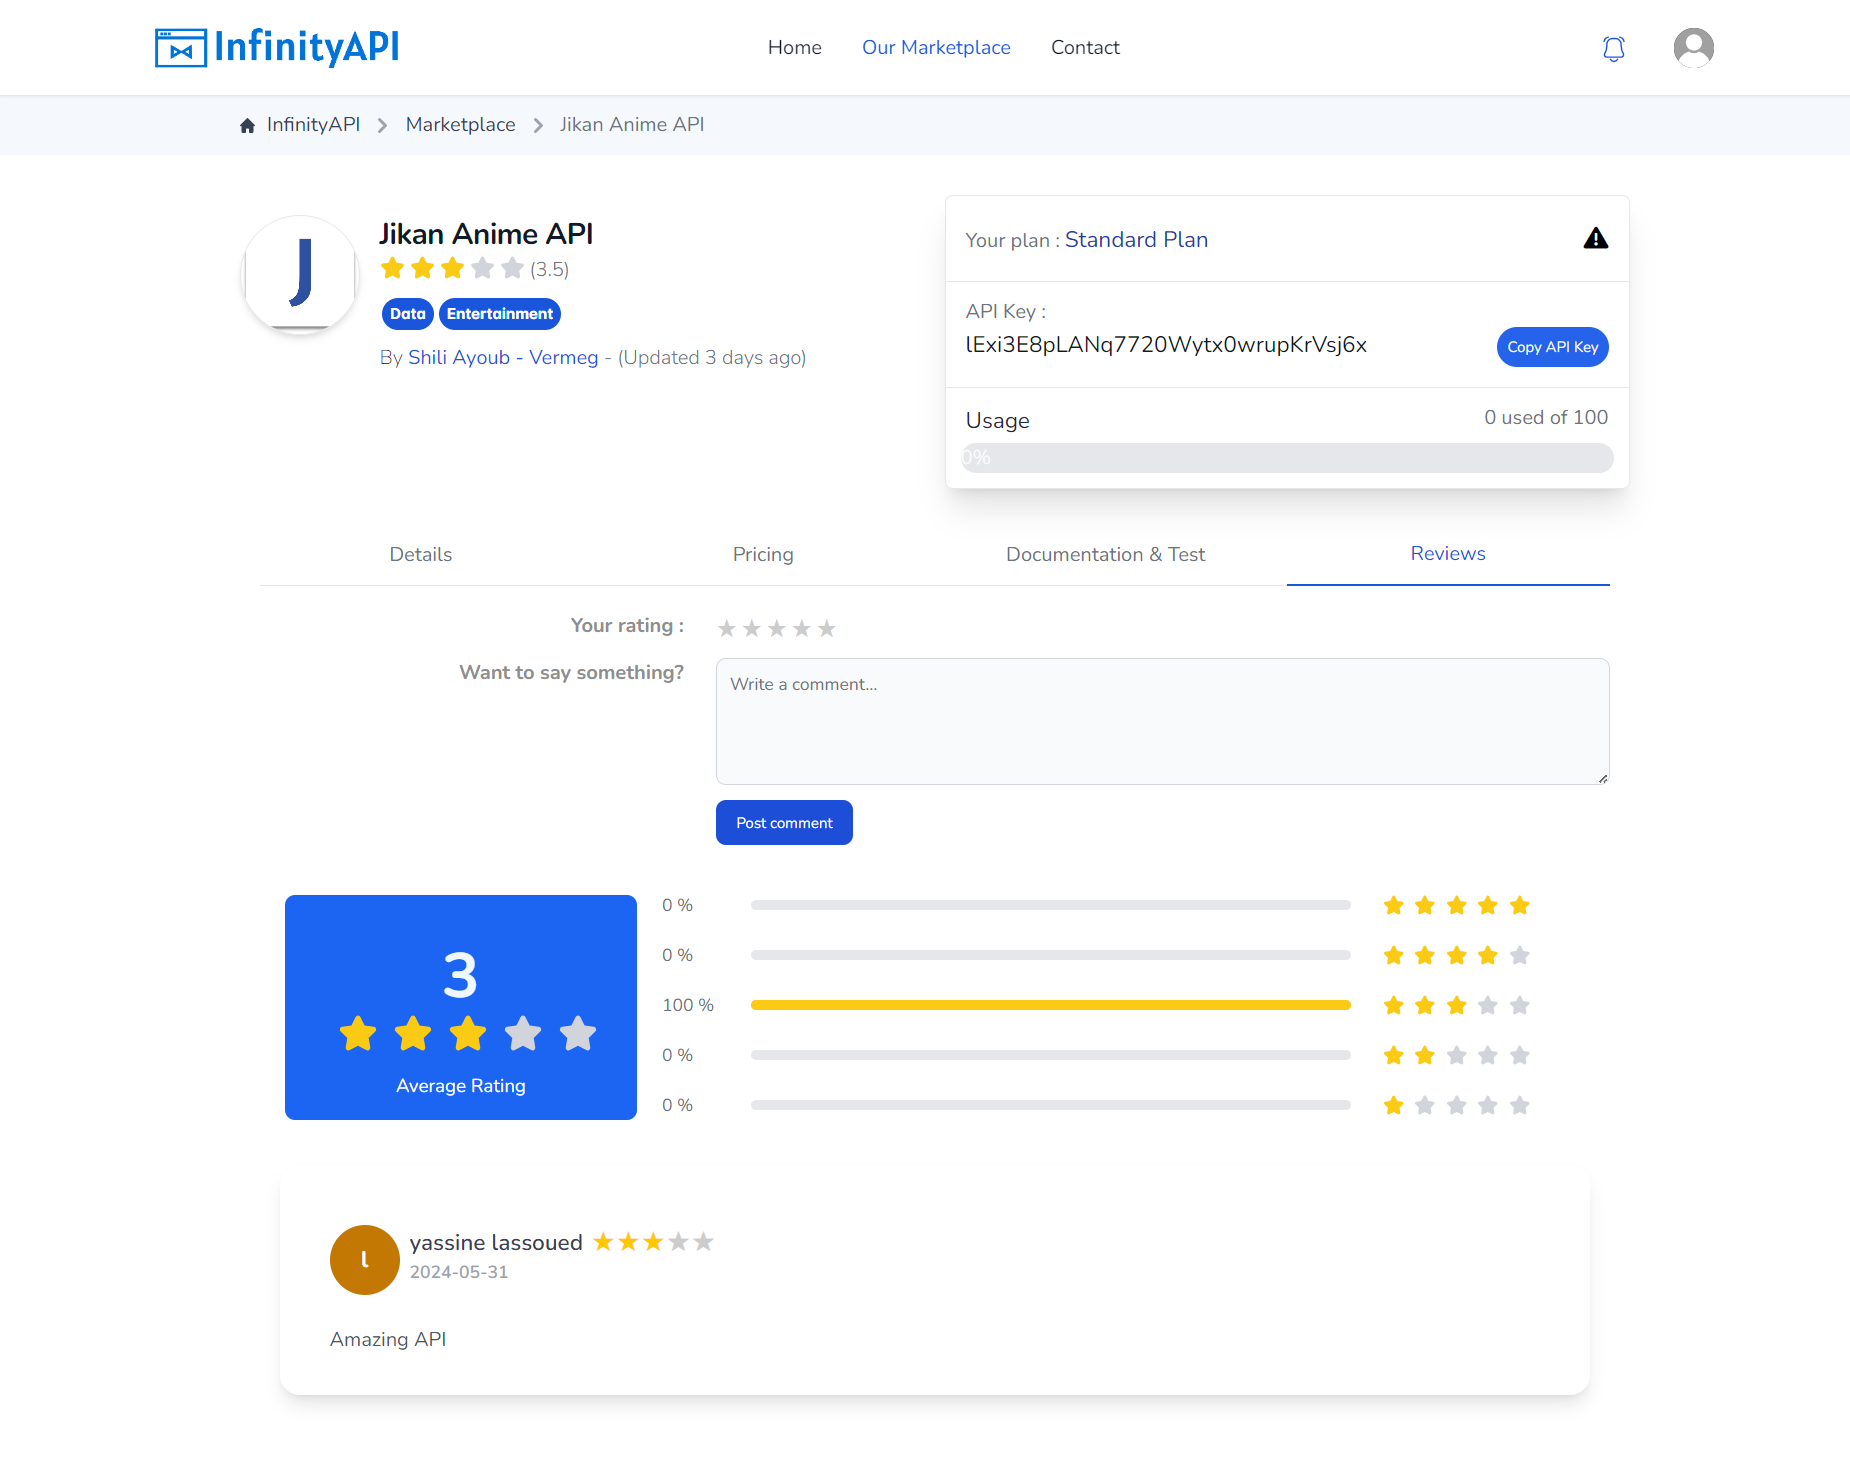
\includegraphics[width=0.8\columnwidth]{   interfacedeprocessusdegestiondunfeedback.png}}
        \caption{ Interface du feedback }
        \label{fig:logo_tt}
    \end{figure}
    \subsubsection{Liste des notifications}

    Cette interface représente la liste des notifications reçu par le développeur en temps réel. 
    \begin{figure}[H]
        \centering
        \frame{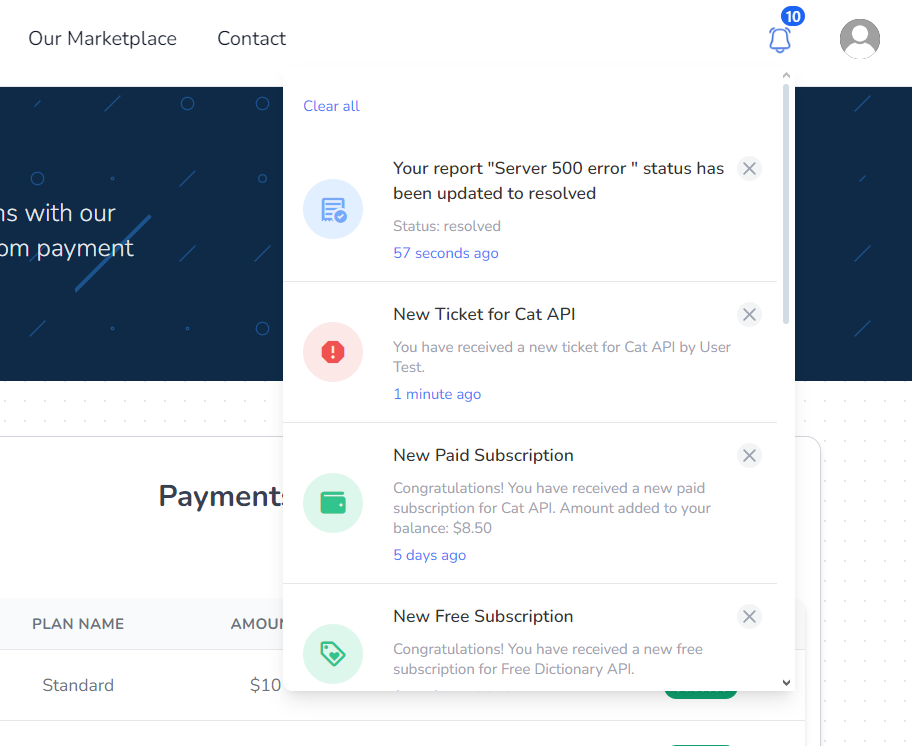
\includegraphics[width=0.8\columnwidth]{  interfacenotification.png }}
        \caption{ Interface de la liste des notifications}
        \label{fig:logo_tt}
    \end{figure}
    
\pagebreak
    \subsection{Burndown Chart}
    \begin{figure}[H]
        \centering
        \frame{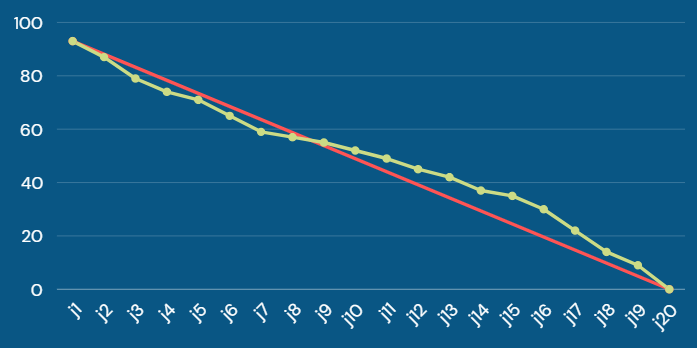
\includegraphics[width=1\columnwidth]{burndownchartsprint3.png}}
        \caption{Burndown chart du sprint 3 }
        \label{fig:logo_tt}
    \end{figure}
    Ce burndown montre que :
    \begin{itemize}
        \item Tous les user stories sont réalisés dans le temps estimé.
        \item La vélocité de notre équipe est 93.
    \end{itemize}
    

    \subsection{Rétrospective du sprint 3}
    \begin{longtable}[c]{|p{0.3\linewidth}|p{0.6\linewidth}|}
        \hline
        \textbf{Les questions} & \textbf{Les réponses} \\
        \hline
        \endfirsthead
        \multicolumn{2}{c}%
        {{\bfseries \tablename\ \thetable{} -- suite de la page précédente}} \\
        \hline
        \textbf{Les questions} & \textbf{Les réponses} \\
        \hline
        \endhead
        \hline \multicolumn{2}{|r|}{{\bfseries Suite à la page suivante}} \\
        \hline
        \endfoot
        \hline
        \endlastfoot
    
        \multirow{2}{=}{Ce qui s'est bien passé} & Achèvement des travaux dans le temps estimé \\
        &Le projet a été validé par le Product Owner\\
        \hline
        \multirow{2}{=}{Les problèmes rencontrés} & Manque de repos \\
        &Difficultés lors de la fusion du code 
      
    \end{longtable}

\section*{Conclusion}
Au cours de ce dernier chapitre, nous avons présenté la spécification fonctionnelle, la conception, ainsi que la revue et la rétrospective de ce dernier sprint. Ce chapitre marque la fin du cycle de développement Scrum, aboutissant à un travail exécutable.
